\documentclass[tikz,border=5pt]{standalone}
\usepackage{amsmath}
\usetikzlibrary{arrows.meta, decorations.markings}

\begin{document}
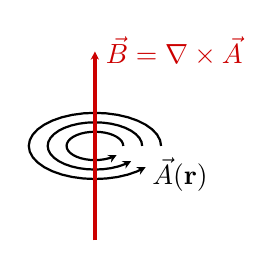
\begin{tikzpicture}[scale=1.2, >={Stealth[length=3pt,width=3pt]}]

% === B-veld als rotatie van A ===
% Vectorpotentiaal A (ronddraaiend)
\foreach \r in {0.3,0.5,0.7}{
  \draw[->,thick,domain=0:320,samples=33] plot ({\r*cos(\x)-0.5},{\r*sin(\x)*0.5-3});
}

% Magnetisch veld B omhoog
\draw[red!80!black,->,very thick] (-0.5,-4) -- (-0.5,-2) node[right] {$\vec{B} = \nabla \times \vec{A}$};

% Labels
\node at (0.4,-3.3) {$\vec{A}(\mathbf{r})$};
\end{tikzpicture}
\end{document}